\chapter{Sprint backlogs and burn down charts}
\label{sec:sprintbacklog}
This appendix contains sprint backlogs and burn down charts for all the sprints.

\section{Sprint 1}
\begin{figure}[H]
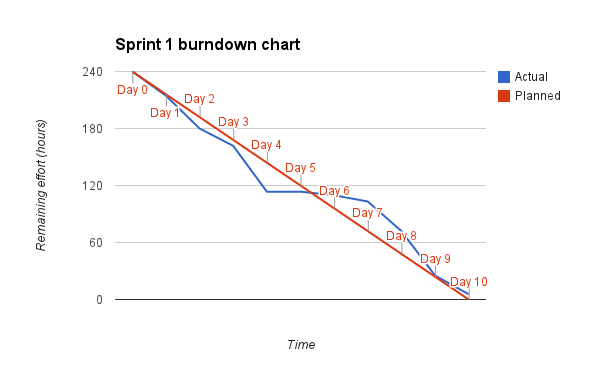
\includegraphics[width=\textwidth]{appendix/backlog/burndown1.png}
\caption{Burn down chart for sprint 1}
\end{figure}
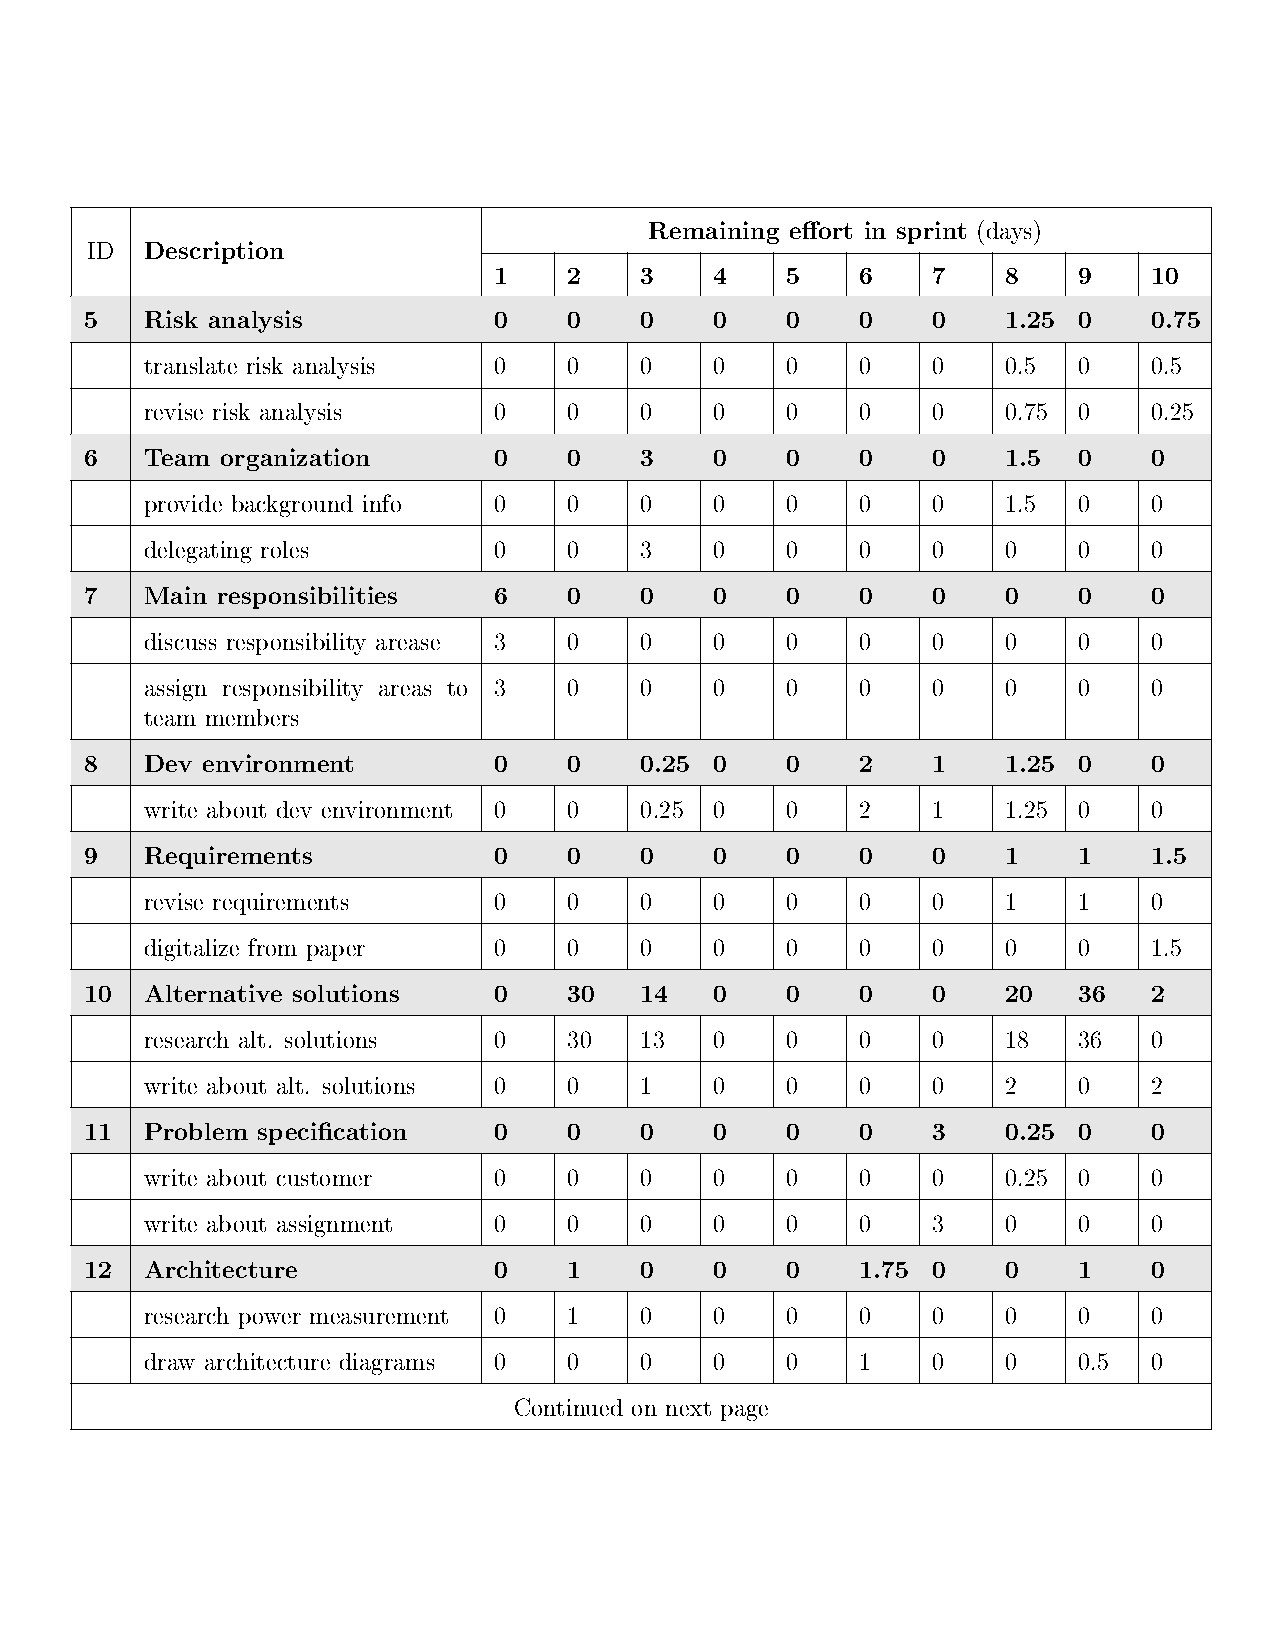
\includepdf[pages=-, scale=0.85]{appendix/backlog/backlog1.pdf}

\section{Sprint 2}
\begin{figure}[H]
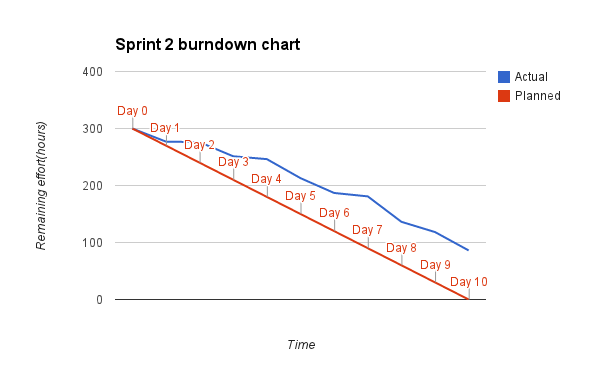
\includegraphics[width=\textwidth]{appendix/backlog/burndown2.png}
\caption{Burn down chart for sprint 2}
\end{figure}
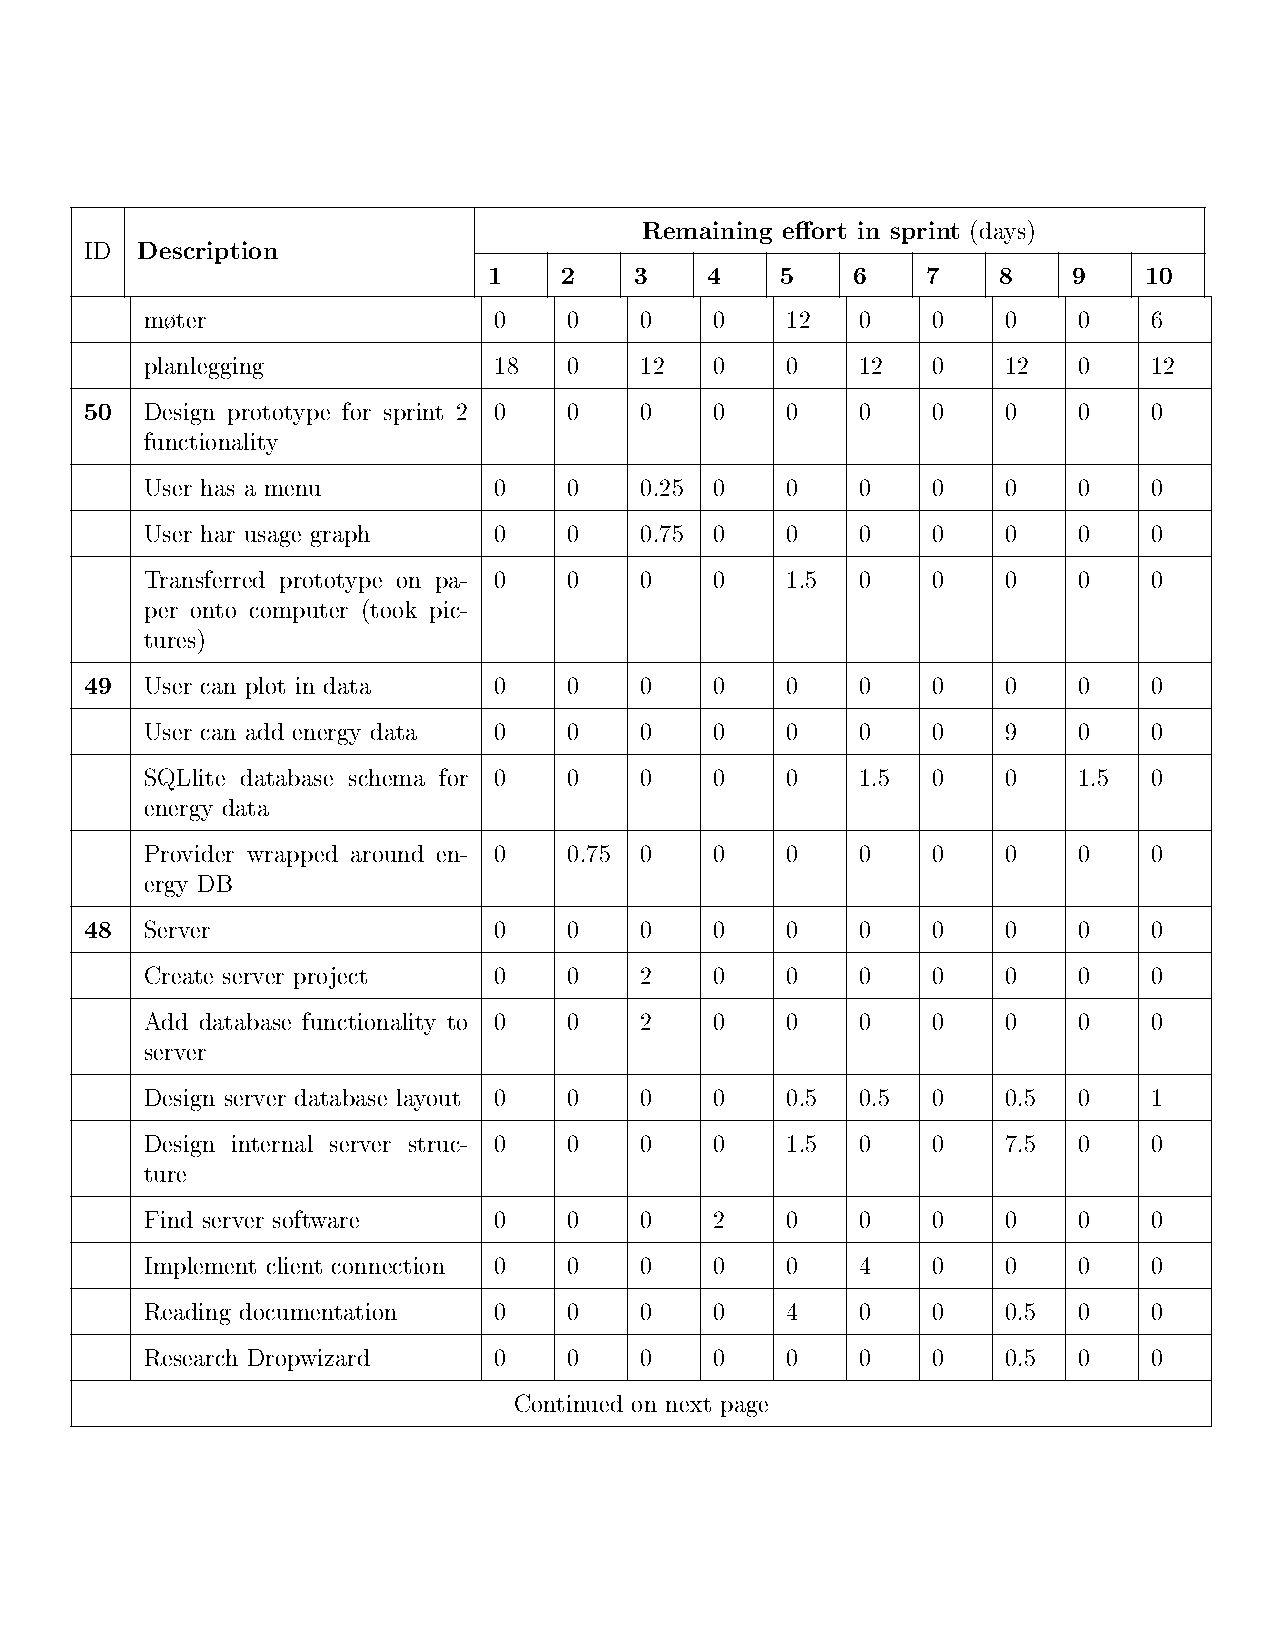
\includepdf[pages=-, scale=0.85]{appendix/backlog/backlog2.pdf}

\section{Sprint 3}
\begin{figure}[H]
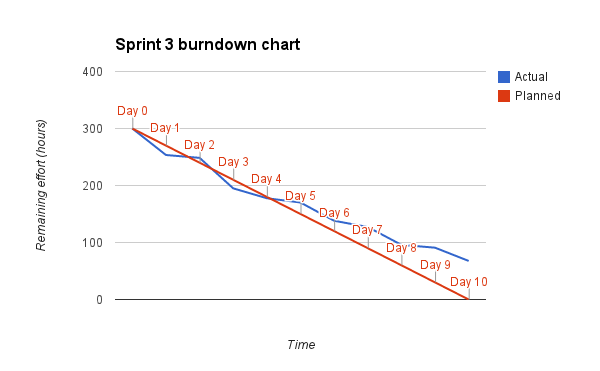
\includegraphics[width=\textwidth]{appendix/backlog/burndown3.png}
\caption{Burn down chart for sprint 3}
\end{figure}
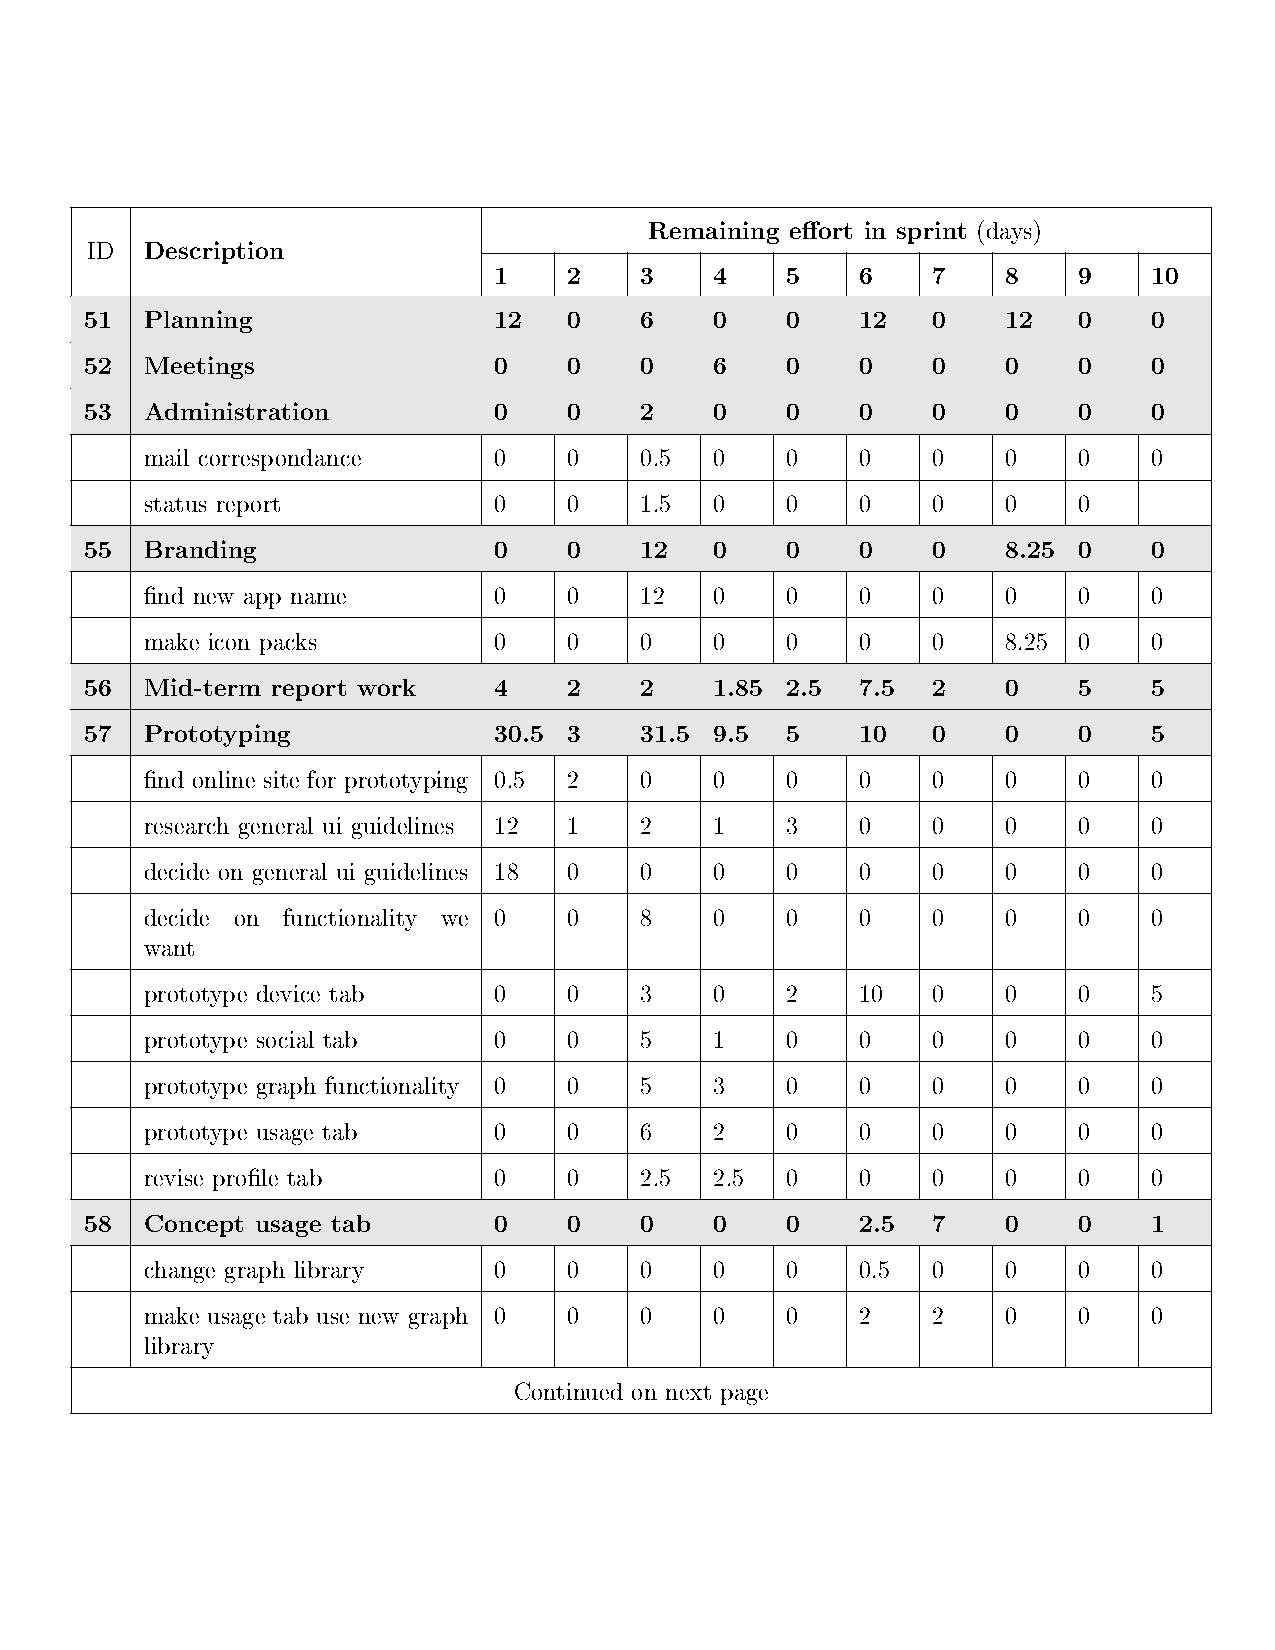
\includepdf[pages=-, scale=0.85]{appendix/backlog/backlog3.pdf}

\section{Sprint 4}
\begin{figure}[H]
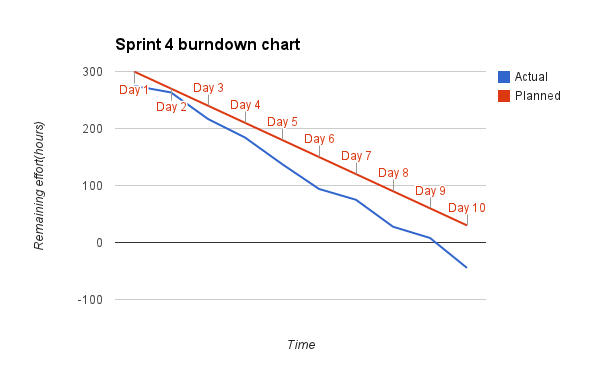
\includegraphics[width=\textwidth]{appendix/backlog/burndown4.png}
\caption{Burn down chart for sprint 4}
\end{figure}
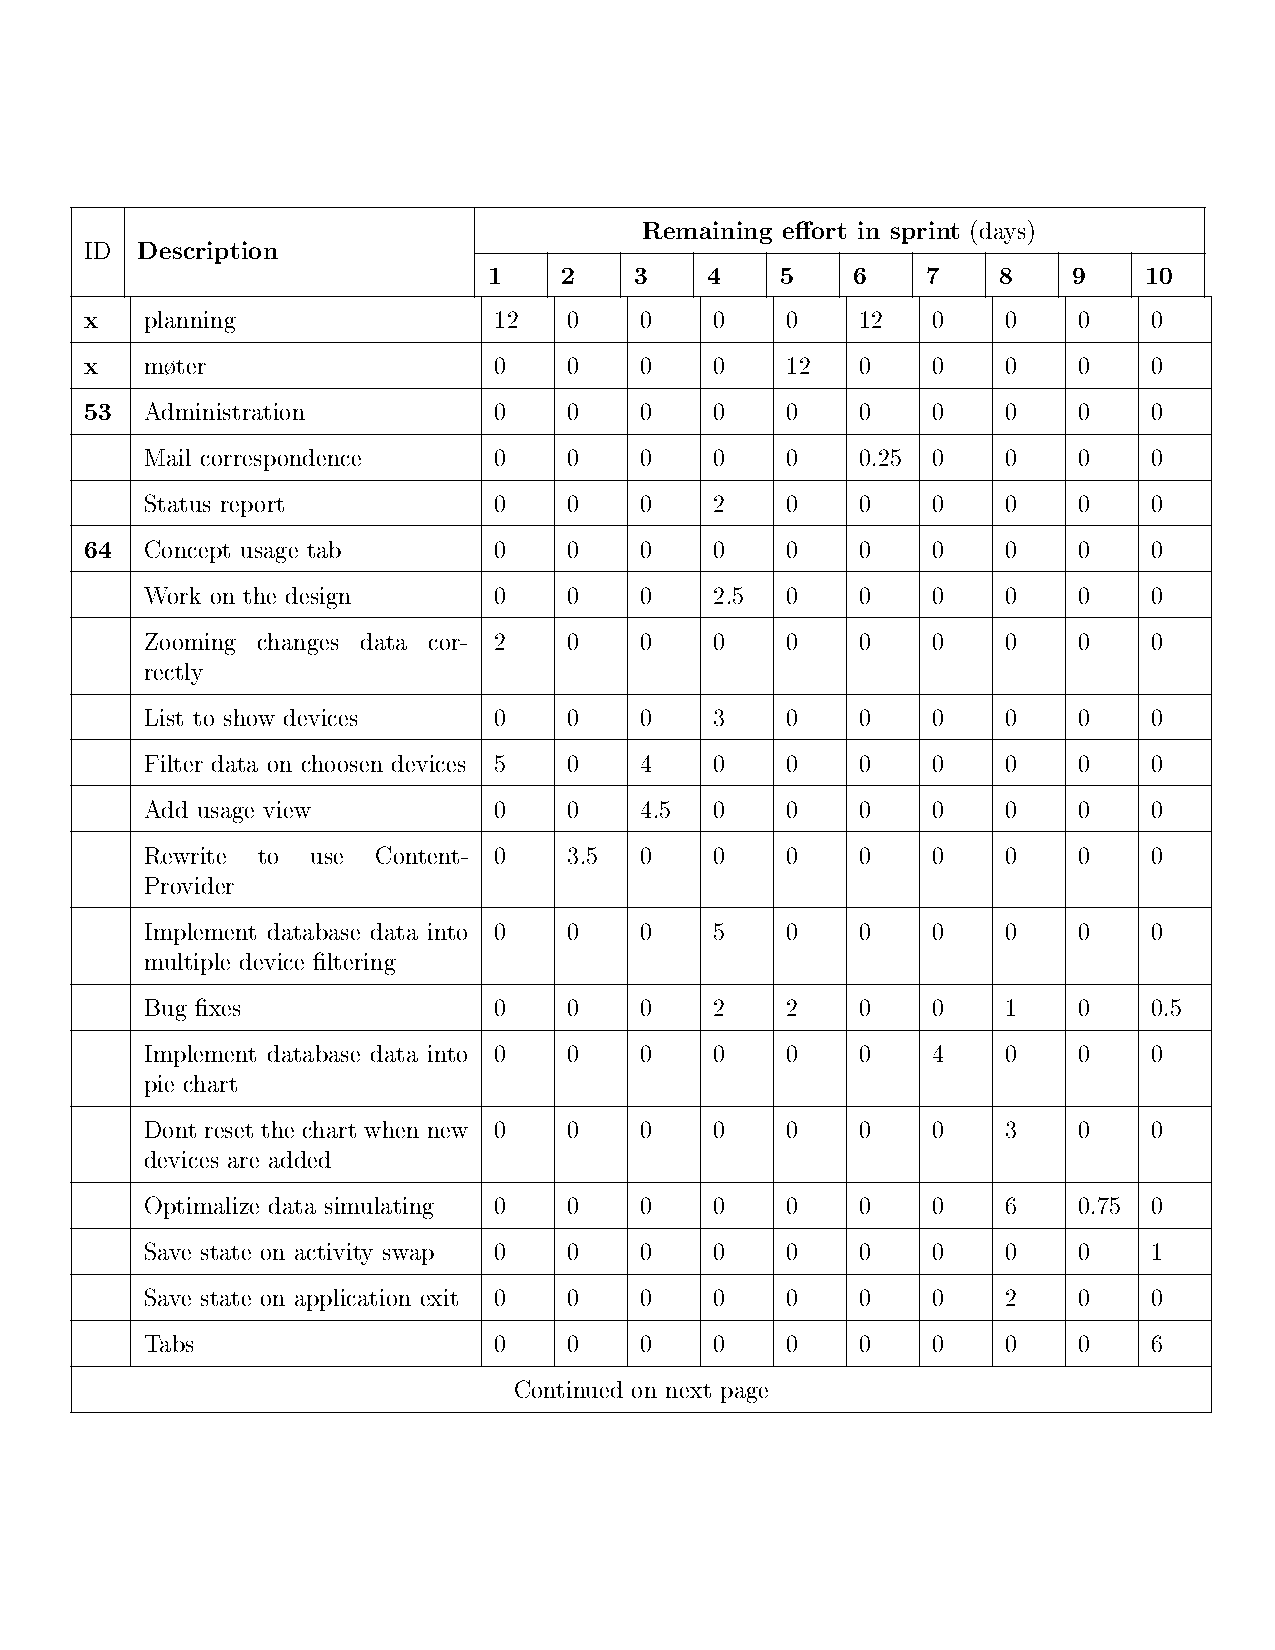
\includepdf[pages=-, scale=0.85]{appendix/backlog/backlog4.pdf}

\section{Sprint 5}
\begin{figure}[H]
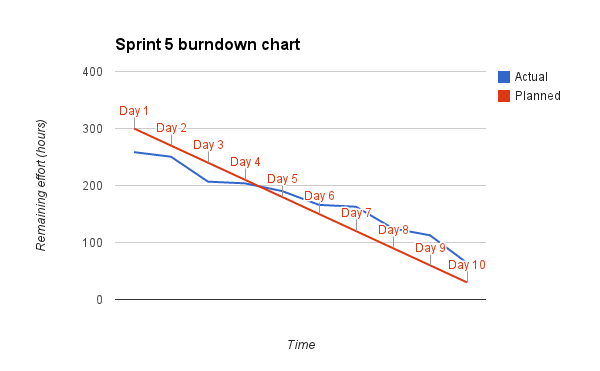
\includegraphics[width=\textwidth]{appendix/backlog/burndown5.png}
\caption{Burn down chart for sprint 5}
\end{figure}
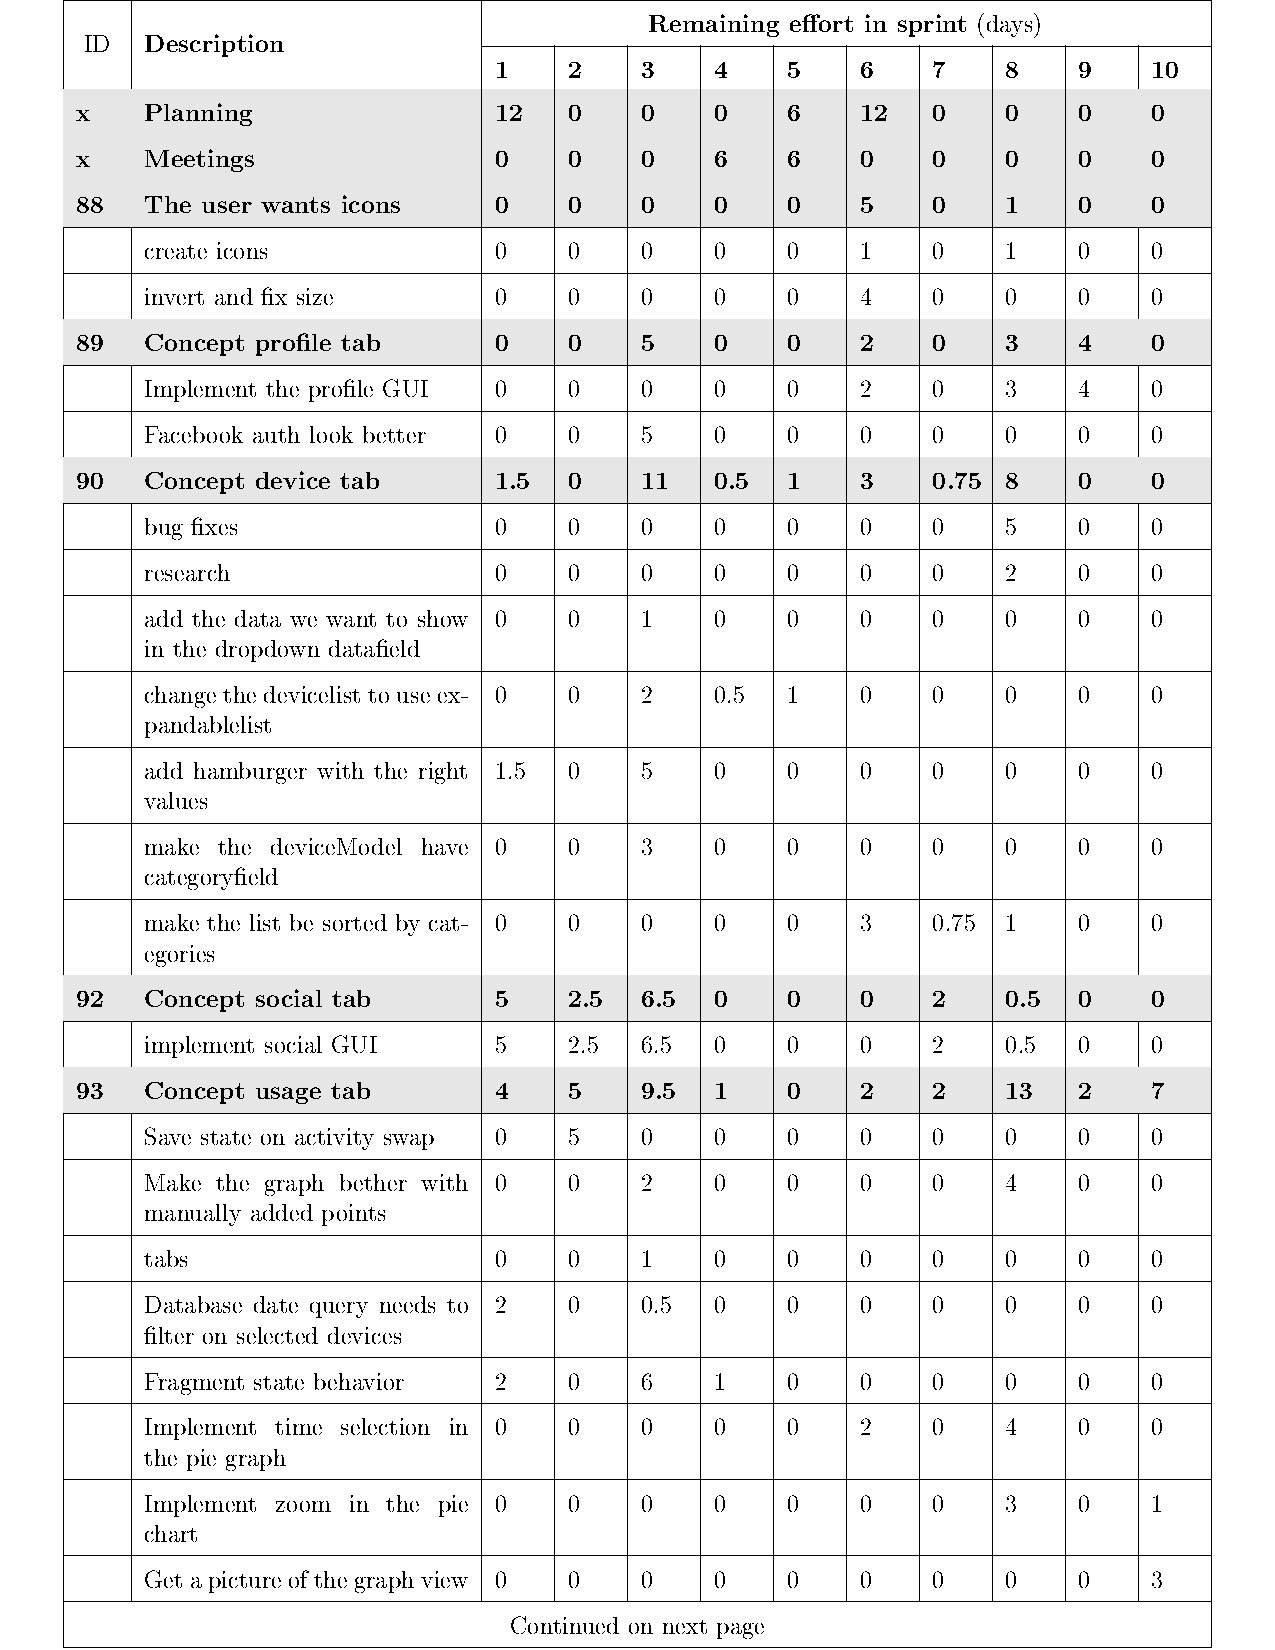
\includepdf[pages=-,scale=0.85]{appendix/backlog/backlog5.pdf}

\section{Sprint 6}
\begin{figure}[H]
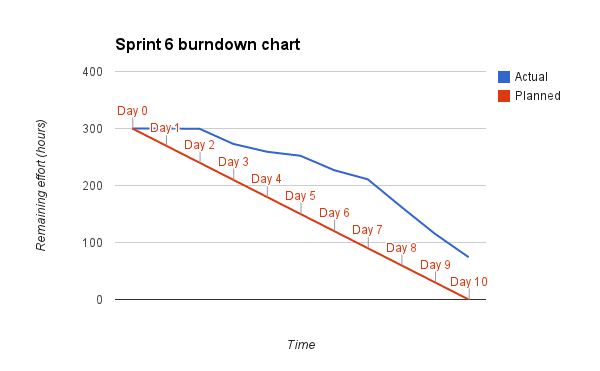
\includegraphics[width=\textwidth]{appendix/backlog/burndown6.png}
\caption{Burn down chart for sprint 6}
\end{figure}
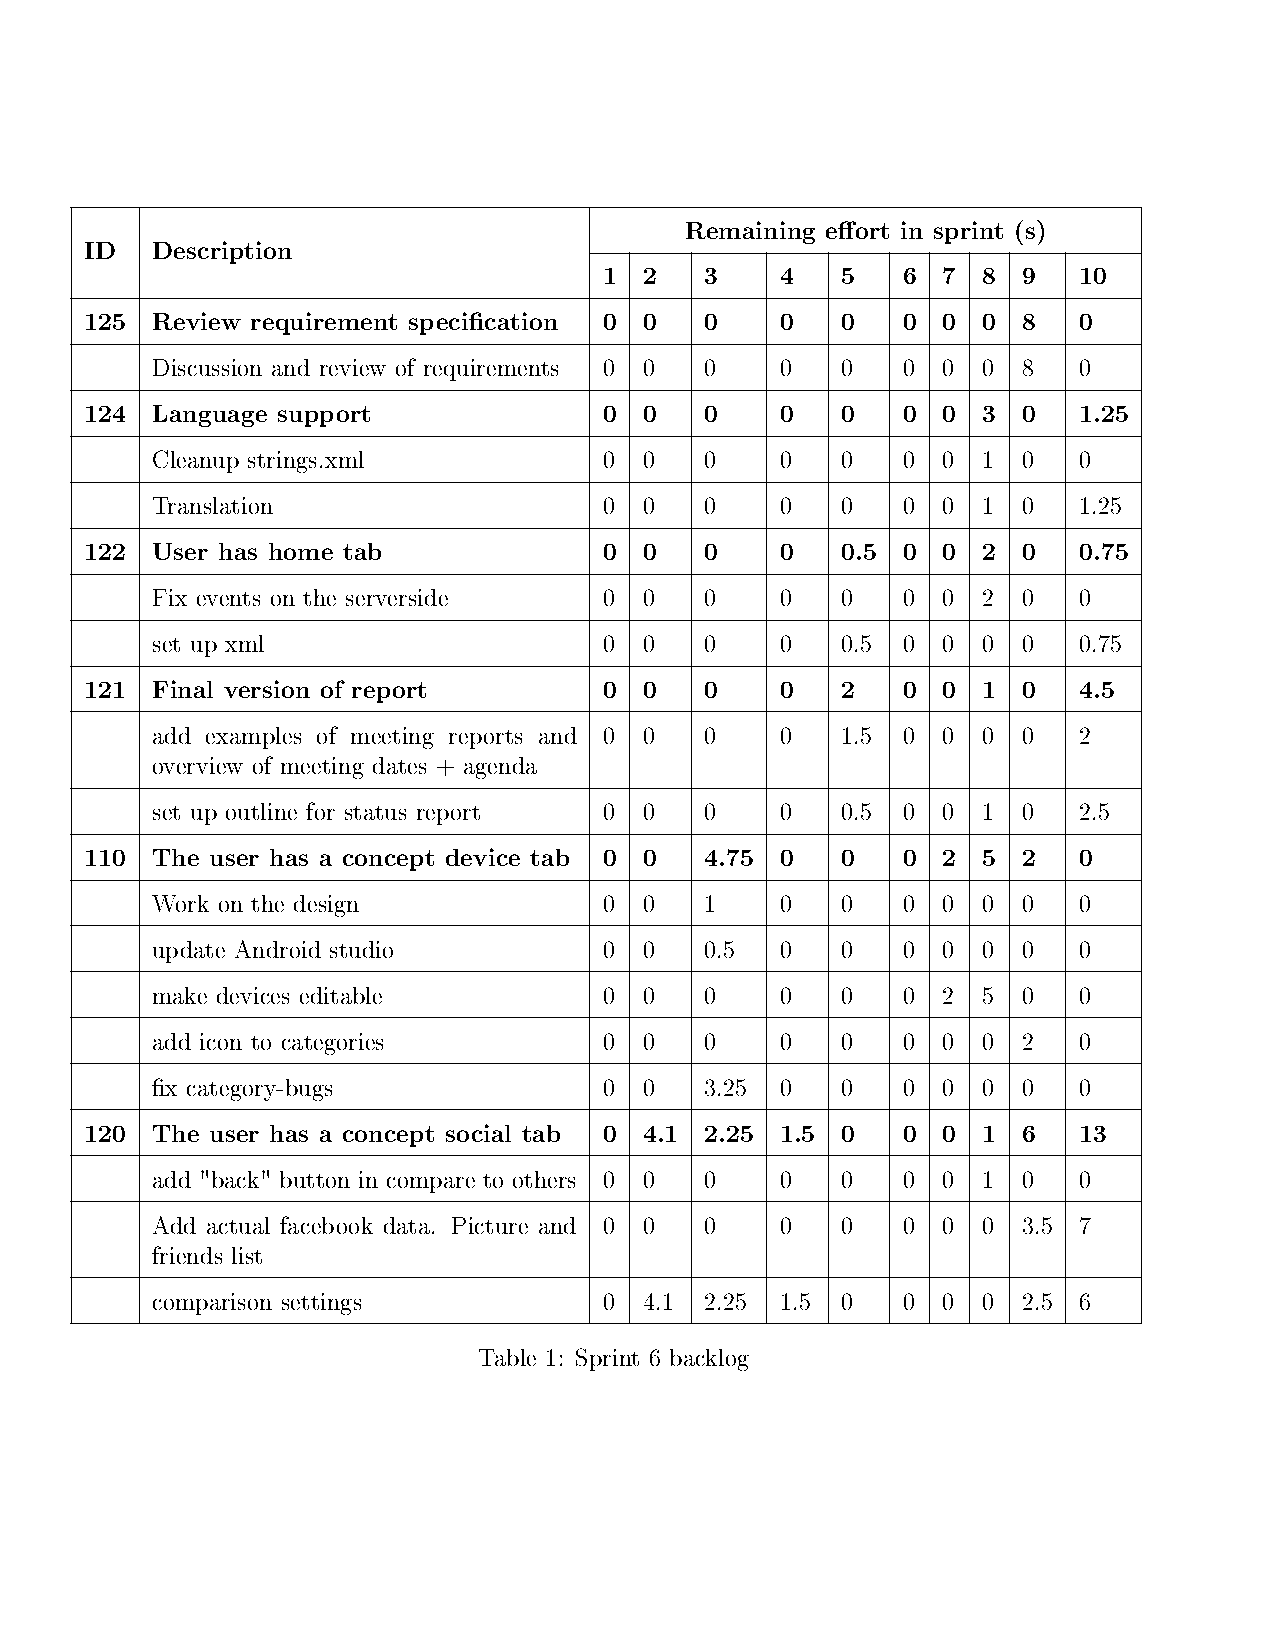
\includepdf[pages=-, scale=0.85]{appendix/backlog/backlog6.pdf}

